\documentclass{article}
\usepackage{graphicx} % Required for inserting images
\usepackage{tikz}
\usepackage{subcaption}
\usetikzlibrary{positioning}
\graphicspath{ {./Pics} }

\title{\textbf{Neural Network for System Identification} \\ -- Project 1}

\author{Enes Erçin}
\date{April 2023}

\begin{document}

\maketitle

\section{Aim}
\textnormal{To train a single layer neural network using any adaptive algorithm, with the input of sinusoidal signals expecting model to predict a function that is close to sinusoidal. For this particular project adaptive algorithm chosen is famous back propagation algorithm. It is important to keep in mind there are infinite amount of different parameter combinations that can be tested, for this document only few of them are investigated. The outcome of the algorithm might be differ with different parameters, this document focuses on the results of the parameters chosen which are showed in parameters section. At the end of the experiment model did predict well defined sinusoidal function although the output seems perfect sinusoidal waveform at first maximum, minimum and mean values are different then the sinusoidal values.}

\section{Features}
\subsection{Parameters}
\textnormal{\begin{table}[ht]
    \centering
    \begin{tabular}{c|c}
     Number of inputs:	                       & 5\\
     \hline
     The frequency of sinusoidal sampling:      & 100\\ 
     \hline
     Adaptive Algorithm:                        & Back propagation\\ 
     \hline
     Non-linear Activation Function:		      & Sigmoid \\
     \hline
     Number of Training Size:	      & 2500\\ 
     \hline
     Learning Rate:                        & 0.001\\ 
     \hline
      Cost Function:                       & Least Squares 
    \end{tabular}
    \caption{Parameters of the Model}
\end{table}}

\subsection{Input}
\paragraph{}
An array is initiated by consecutive numbers with the difference of defined sampling rate a \( a = 2\pi/sample freq\) . After that array is used as an input for sinusoidal function \( sin(a*t) \).  For each training sequence first five of values of the array is chosen as input and the next one namely sixth data is chosen as expected value. Then second training starts with second value of the array and expected value for this case chosen as seventh value of the array.
\paragraph{}
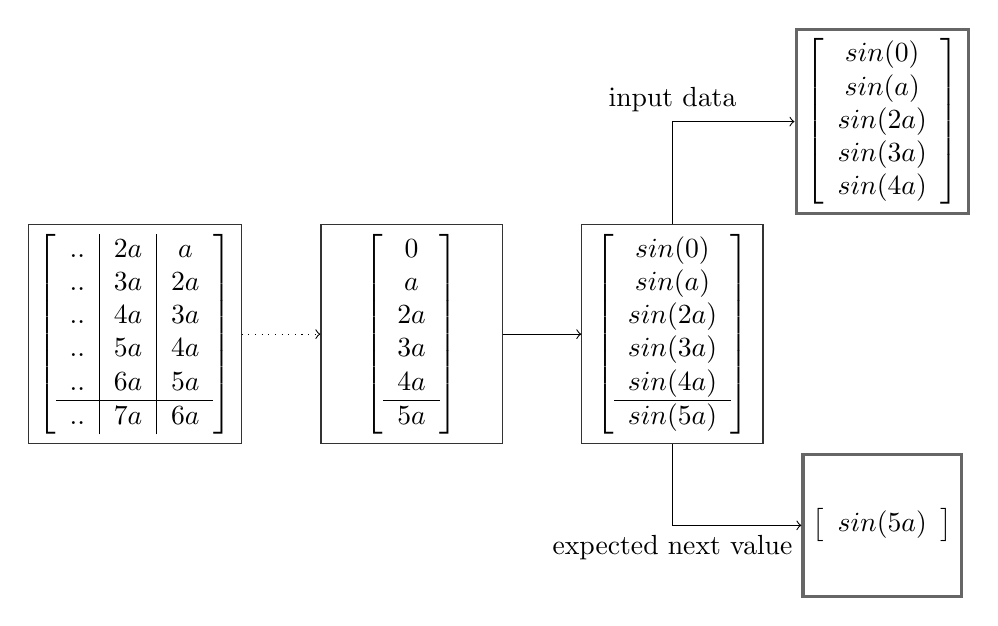
\begin{tikzpicture}[
roundnode/.style={rectangle,draw=black!80, minimum size=23mm},
dimondnode/.style={rectangle, draw=black!60, very thick, minimum size=18mm},
placeholder/.style={minimum size=10mm},
]
%Nodes
\node[roundnode]        (store)      {$\left[ \begin{array}{c|c|c}
        ..&2a&a\\
        ..&3a&2a\\
        ..&4a&3a\\
        ..&5a&4a\\
        ..&6a&5a\\
        \hline
        ..&7a&6a\\
        \end{array}\right]$};

        
\node[roundnode]        (init)  [right=of store]      {$\left[ \begin{array}{c}
        0\\
        a\\
        2a\\
        3a\\
        4a\\
        \hline
        5a\\
        \end{array}\right]$};
        
\node[roundnode]        (funct)       [right=of init] {$\left[ \begin{array}{c}
        sin(0)\\ 
        sin(a)\\ 
        sin(2a)\\ 
        sin(3a)\\ 
        sin(4a)\\
        \hline
        sin(5a)\\
\end{array}\right]$};

\node [placeholder] (placeholder) [right=of funct] {};
\node[dimondnode]        (input)       [above=of placeholder] {$\left[ \begin{array}{c}
        sin(0)\\ 
        sin(a)\\ 
        sin(2a)\\ 
        sin(3a)\\ 
        sin(4a)\\
\end{array}\right]$};

\node[dimondnode]        (ref)       [below=of placeholder] {$\left[ \begin{array}{c}
        sin(5a)\\
\end{array}\right]$};

%Lines
%Lines
\draw[->] (funct.north) |- (input.west)node [midway, above] (TextNode) {input data};
\draw[->] (funct.south) |- (ref.west)node [midway, below] (TextNode) {expected next value};;
\draw[->] (init.east)  -- (funct.west);
\draw[->][dotted] (store.east) -- (init.west);
    
\end{tikzpicture}

\subsection{Adaptive Algorithm: Back propagation}
\paragraph{}
The concept of adaptive algorithms responsibility is to find the optimal parameters that will reduce the cost function. In this model of basic neural network it is only possible to change weights and biases. The process of defining a change value for bias and weights comes from particular choice of adaptive algorithm. In this project chosen adaptive algorithm is back propagation.  Mindset behind the algorithm is simple there is a function that we want to reduce to its minimum value. That function is cost function. For every input we would get a different set of cost function results. 
\[ J(\theta) = \sum_{n=0}^{n=k}[y(\theta_n) -d)]^2 \]
Since only parameter that are possible to change are weights and biases we must find its partial derivative with respect to cost function. To find \( dJ(\theta)/dw,  dJ(x)/db\) values chain rule must be applied. 
\[  y_n=y(\theta_n)  = \sigma(w_n*\theta_n + b_n) \]
Lets say = \(a_n = \sigma(w_n*\theta_n + b_n))\)  for ease of representation.
\[  \frac{dJ(\theta_n)}{dw_n} =  \frac{dJ(\theta_n)}{y_n} \cdot \frac{dy_n}{da_n} \cdot  \frac{da_n}{dw_n} \]
Similarly, also noticing that  \( \frac{da_n}{db_n} \) = 1
\[  \frac{dJ(\theta_n)}{db_n} =  \frac{dJ(\theta_n)}{y_n} \cdot \frac{dy_n}{da_n} \]
It is a common practice to pick a learning rate which is close to 0 so that the most optimum weights and biases can be reached within reasonable speed. Basically smaller learning rates can give higher precision while gives a slower progress. It is also important to keep in mind it is possible to change the learning rate while training. Approach names ad adaptive learning rate. For this practice picked learning rate is 0.001. Thus weight and biases are adjusted with given formula.
\[  w_n[1] =  w_n[0] - 0.001 \cdot \frac{dJ(\theta_n)}{dw_n}\]
\subsubsection{Code}

\begin{figure}[h]
    \includegraphics[width=1\linewidth, height=8cm ]{pics/backpropcode.png}
    \caption{Caption}
    \label{fig:my_label}
\end{figure}

\begin{figure}[h]
    \includegraphics[width=1\linewidth, height=12cm ]{pics/forwardprop_code.png}
    \caption{Caption}
    \label{fig:my_label}
\end{figure}
\section{Results}
\paragraph{}
A function close to sinusoidal is estimated at the end of the epochs however maximum and minimum values of the estimated sinusoidal-like function is not -1 and 1 rather its 2-0. Although this value of estimation can change depending on different parameters it is not straight forward to say why it did not give a closer result. 
\begin{figure}[h]
    \includegraphics[width=0.9\linewidth, height=10cm]{pics/results.png}
    \caption{Results with defined parameters. 1-Expected Value 2-Returned Value 3-Return and expected values}
    \label{fig:my_label}
\end{figure}

\begin{figure}[h]

\begin{subfigure}{0.5\textwidth}
    \includegraphics[width=0.99\linewidth, height=5cm]{pics/aa.png}
    \caption{Weigths over time}
    \label{fig:my_label}
\end{subfigure}
\begin{subfigure}{0.5\textwidth}
    \includegraphics[width=0.99\linewidth, height=5cm]{pics/bb.png}
    \caption{Loss value over time}
    \label{fig:subim2}
\end{subfigure}

\caption{Changes of the neuron parameters over time}
\label{fig:image2}
\end{figure}


\begin{figure}[h]
    \centering
    \includegraphics[width=0.9\linewidth, height=10cm]{pics/results_2.jpg}
    \caption{Results with lower sampling rate. 1-Expected Value 2-Returned Value 3-Return and expected values}
    \label{fig:my_label}
\end{figure}

\end{document}
